\documentclass[a4paper,12pt]{scrartcl}
\usepackage[utf8]{inputenc}
\usepackage[ngerman]{babel}
\usepackage[T1]{fontenc}
\usepackage{amsmath}
\usepackage{stmaryrd}
\usepackage{wasysym}
\usepackage{lmodern}
\usepackage{graphicx}
\usepackage{paralist}
\usepackage{upgreek}
\usepackage{subfigure}
\usepackage{tipa}
\usepackage{amssymb}
\usepackage{gensymb}
\usepackage{dsfont}
\usepackage{mathtools}
\usepackage{ stmaryrd }
\usepackage{fancyhdr}
\usepackage{tikz}
\usetikzlibrary{arrows,automata}

%\title{Abgabe 1}
%\author{Rafael Heid, Julian Deinert, Sabrina Buczko Gruppe\\ 6 und 7}
%\date{Abgabe am 24.10.16}

\gdef\blatt{FGI-2 Aufgabenblatt 08}

\title{\blatt}
\date{Gruppe 06}
\author{Sabrina Buczko 6663234, Julian Deinert 6535880, Rafael Heid 6704828}


\pagestyle{fancy}
\fancyhf{}
\fancyhead[L]{\blatt}
\fancyhead[R]{Buczko, Deinert, Heid}
\fancyfoot[C]{\thepage}

\begin{document}
\maketitle
\newpage
\setcounter{section}{7}
% Section 7
\section{}
\setcounter{subsection}{2}
% Section 7.3
\subsection{}
\subsubsection{}
\begin{tikzpicture}[->,>=stealth',shorten >=1pt,auto,node distance=3cm, semithick]
  \tikzstyle{every state}=[fill=none,draw=none,text=black]

  \node[state] (A)              {$p1(2)$};
  \node[state] (B) [right of=A] {$p1p2$};
  \node[state] (C) [below of=B] {$p2p3$};
  \node[state] (D) [right of=B] {$p2(2)$};
  \node[state] (E) [below of=D] {$p2p5$};
  \node[state] (F) [below of=A] {$p1p3$};
  \node[state] (G) [below of=E] {$p4p5$};
  \node[state] (H) [below of=C] {$p3p4$};
  \node[state] (I) [below of=F] {$p3(2)$};
  \node[state] (J) [below of=H] {$p3p6$};
  \node[state] (K) [below of=G] {$p5p6$};
  \node[state] (L) [right of=E] {$p2p6$};
  \node[state] (M) [below of=L] {$p4p6$};
  \node[state] (N) [right of=D] {$p2p4$};
  \node[state] (O) [below of=K] {$p5(2)$};
  \node[state] (P) [below of=J] {$p3p5$};
  \node[state] (Q) [below of=M] {$p6(2)$};
  \node[state] (R) [right of=M] {$p4(2)$};
     

  \path (A) edge              node {$t_1$} (B)
  		(A) edge			  node {$t_2$} (F)
        (B) edge              node {$t_1$} (D)
            edge              node {$t_2$} (C)
        (C) edge              node {$t_3$} (A)
        (E) edge 			  node {$t_6$} (C)
        (F) edge              node {$t_1$} (C)
        	edge              node {$t_2$} (I)
        (C) edge              node {$t_4$} (G)
        (G) edge              node {$t_5$} (E)
        	edge              node {$t_6$} (H)
        	edge              node {$t_7$} (Q)
        (H) edge              node {$t_5$} (C)
        (J) edge              node {$t_8$} (H)
        	edge              node {$t_9$} (P)
        (K) edge              node {$t_6$} (J)
        	edge              node {$t_8$} (G)
        	edge              node {$t_9$} (O)
        (L) edge              node {$t_9$} (E)
        	edge              node {$t_8$} (N)
        (M) edge              node {$t_9$} (G)
        (N) edge              node {$t_5$} (D)
        (O) edge              node {$t_6$} (P)
        (P) edge              node {$t_6$} (I)
        (Q) edge              node {$t_8$} (M)
        	edge              node {$t_9$} (K)
        (M) edge              node {$t_8$} (R)
        (R) edge [bend right]           node {$t_5$} (N);
  
        
\end{tikzpicture}
%Anhand des Erreichbarkeitsgraphen ist zu erkennen, dass das Netz \textbf{nicht reversibel} ist, da $m_0$ in $p_1$ von allen weiteren erreichbaren Markierungen aus erreichbar ist. Ebenso ist es \textbf{lebendig}, da jede Transition in jeder Markierung potenziell aktivierbar ist und es keine Verklemmungen gibt. Es ist auch \textbf{beschränkt}, da der Graph endlich ist.\\\\%
\\
\textbf{Lebendigkeit:} Das Netz ist nicht Lebendig,
da aus der Markierung $p3(2)$ heraus keine Markierung 
erreicht werden kann die eine beliebige Transition 
aktiviert.\\
\textbf{Reversibilität:} Das Netz ist nicht reversibel, da mit der Schaltfolge\\
$p1(2) \xrightarrow{t_2} p1p3 \xrightarrow{t_2} p3(2)$
\\
eine Markierung erreicht werden kann, aus der die 
Anfangsmarkierung nicht mehr zu erreichen ist.\\
\textbf{Beschränktheit:} Das Netz ist 2-beschränkt, da 
der Erreichbarkeitsgraph zeigt, dass nie mehr als 2 
Marken auf einem Platz liegen.\\
\textbf{Strukturelle Eigenschaften:\\}
\subsubsection{}
\textbf{Strukturelle Beschränktheit:}\\
\textbf{Strukturelle Lebendigkeit:}\\
\textbf{Fairness: }Das Netz schaltet nicht fair, da 
z.b. von Markierung $p_2 p_3$ aus die beiden Marken 
nur reichen um entweder den Pfad $t_3$ zu gehen oder 
den Pfad $t_4$. Es gibt also unfaire Folgen in diesem 
Netz. Also müssen nicht alle Transitionen immer 
schalten, was für Fairness eine Voraussetzung ist.
\subsubsection{}
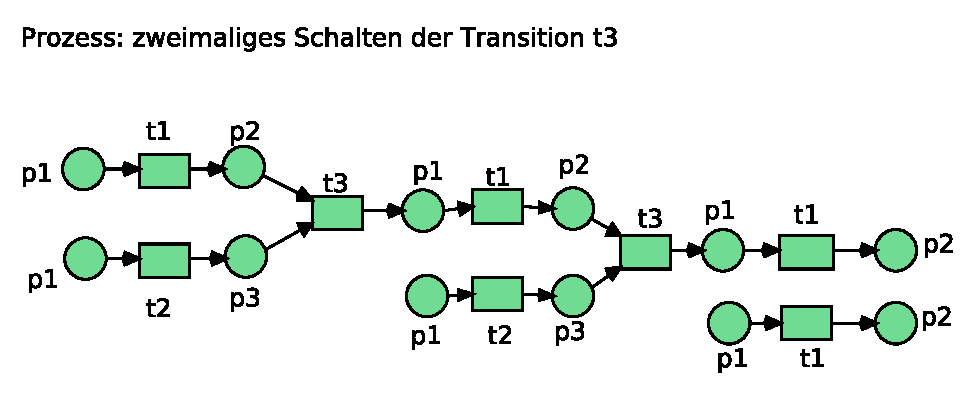
\includegraphics[scale=0.8]{G-6-A-08-Netz1-Buczko_Heid_Deinert.pdf}\\
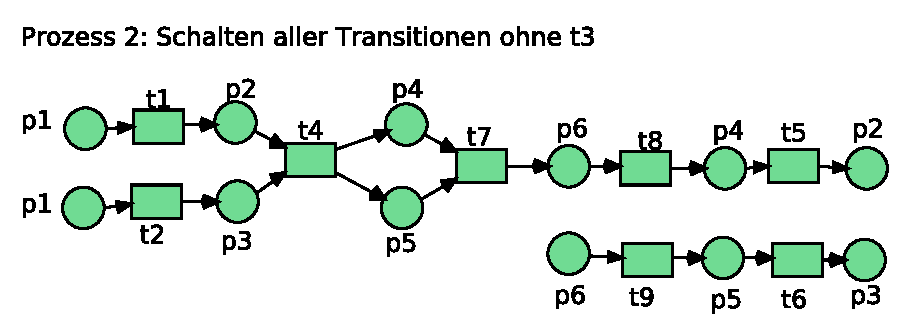
\includegraphics[scale=0.8]{G-6-A-08-Netz2-Buczko_Heid_Deinert.pdf}\\
\subsubsection{}
1. P-Schnitt: Zusammenfassen der Plätze p2 und p3.\\
2. P-Schnitt: Zusammenfassen der Plätze p4 und p5.\\\\
1. T-Schnitt: Zusammenfassen der Transitionen t1 und t2.\\
2. T-Schnitt: Zusammenfassen der Transitionen t8 und t9.\\\\
1. allgemeiner Schnitt: Zusammenfassen der Elemente p1, t1 und p2.\\
2. allgemeiner Schnitt: Zusammenfassen der Elemente p1, t2 und p3.\\\\
$\phi^{-1}(t1)$ und $\phi^{-1}(t6)$ können nicht in einem Schnitt liegen, da die Transitionen nicht nebenläufig sind.\\
Schnitte mit einer Transition kann es geben, sie ergeben allerdings keinen Sinn, da sie genau das Verhalten vom vorherigen Netz widerspiegeln.
\subsection{}
\textbf{1. Erreichbarkeitsgraph zeichnen}\\
\begin{tikzpicture}[->,>=stealth',shorten >=1pt,auto,node distance=3cm, semithick]
  \tikzstyle{every state}=[fill=none,draw=none,text=black]

  \node[state] (A)              {$p1(2)$};
  \node[state] (B) [right of=A] {$p1p2(3)$};
  \node[state] (C) [below of=A] {$p1p2(2)p3$};
  \node[state] (D) [right of=B] {$p2(6)$};
  \node[state] (E) [below of=D] {$p2(5)p3$};
  \node[state] (F) [below of=B] {$p2(4)p3(2)$};
  \node[state] (G) [below of=C] {$p1p2(2)$};
  \node[state] (H) [below of=G] {$p2(5)$};
  \node[state] (I) [right of=H] {$p2(4)p3$};
  \node[state] (J) [below of=F] {$p2(3)p3(3)$};
  \node[state] (K) [below of=E] {$p2(2)p3(4)$};
  \node[state] (L) [below of=K] {$p1p2p3(2)$};
  \node[state] (M) [right of=K] {$p1p3(3)$};
  \node[state] (N) [below of=I] {$p2(3)p3(2)$};
  \node[state] (O) [below of=L] {$p1p2p3$};
  \node[state] (P) [below of=O] {$p1p2$};
  \node[state] (Q) [right of=P] {$p2(4)$};
  \node[state] (R) [right of=O] {$p2(3)p3$};
  \node[state] (S) [right of=L] {$p2(2)p3(2)$};
  \node[state] (T) [right of=M] {$p1p3(2)$};
  \node[state] (U) [right of=S] {$p1p3$};
  
  \node[state] (W) [below of=U] {$p1$};
  \node[state] (X) [right of=W] {$p2(3)$};
  \node[state] (Z) [below of=W] {$p2(2)p3$};
\node[state] (V) [below of=Z] {$p2(2)p3(3)$};
   
  

  \path (A) edge              node {$c$} (B)
        (B) edge              node {$d$} (C)
            edge              node {$c$} (D)
        (C) edge              node {$b$} (A)
        	edge              node {$a$} (G)
        (D) edge              node {$d$} (E)
        (E) edge              node {$b$} (B)
        	edge              node {$d$} (F)
        (F) edge              node {$b$} (C)
        	edge              node {$d$} (J)
        (G) edge              node {$c$} (H)
        (H) edge              node {$d$} (I)
        (I) edge              node {$b$} (G)
        	edge              node {$d$} (N)
        (J) edge              node {$d$} (K)
        	edge              node {$b$} (L)
        (K) edge              node {$b$} (M)
        (L) edge              node {$a$} (O)
        (M) edge              node {$a$} (T)
        (N) edge              node {$b$} (O)
        	edge          [bend right]    node {$d$} (V)
        (O) edge              node {$a$} (P)
        (P) edge              node {$c$} (Q)
        (Q) edge              node {$d$} (R)
        (R) edge              node {$d$} (S)
        	edge  node {$b$} (P)
        (S) edge              node {$b$} (U)
        (T) edge              node {$a$} (U)
        (U) edge              node {$a$} (W)
        (W) edge              node {$c$} (X)
        (X) edge              node {$d$} (Z)
        (Z) edge              node {$b$} (W)
        (V) edge      [bend right=100]        node {$b$} (T);
\end{tikzpicture}
\textbf{2. SZKs finden}\\
\textbf{3. terminale SZKs finden}\\
Zu den terminalen SZKs gehört nur der Zyklus mit den Markierungen $p_1$, $p_2 (3)$, und $p_2 (2)p_3$.\\
\textbf{4. Prüfe für jede terminale SZK, ob es ein m' enthält, dass das Prädikat erfüllt.} \\
In der einzigen terminalen SZK kann man von den drei Markierungen $p_1$, $p_2 (3)$,$p_2 (2)p_3$ in kein m' gelangen in der Transition a aktivierbar ist. Also ist a nicht lebendig. Die Transitionen b,c und d hingegen sind von jeder m erreichbaren m' aktivierbar und somit auch in unserer terminalen SZK aktivierbar. Also sind b,c und d lebendig.
% 8.5
\subsection{}
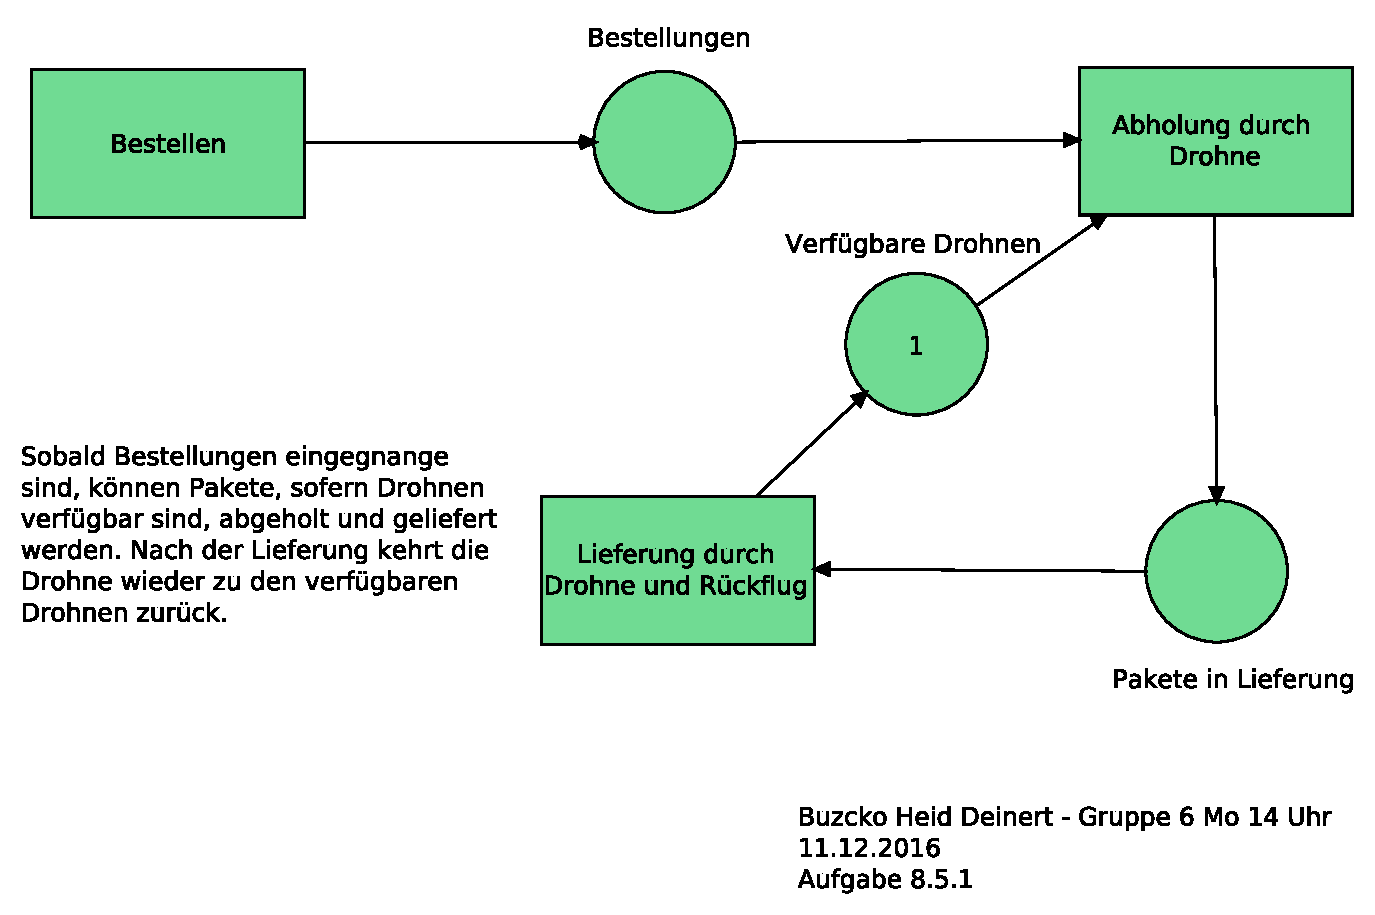
\includegraphics[scale=0.5]{G-6-A-08-Netz3-Buczko_Heid_Deinert.pdf}
% 8.6
\subsection{}
Angenommen N besitzt die Siphon/Trap-Eigenschaft, dann aktiviert jede erreichbare Markierung...?
\begin{itemize}
\item{mind. eine Transition}
\item{höchstens eine Transition}
\item{keine Transition}
\item{beliebig viele Transitionen}
\end{itemize}
Wenn Petrinetze so mächtig wie Turing-Maschinen wären, hätte dies den Nachteil, dass Beschränktheit, Erreichbarkeit und Lebendigkeit nicht entscheidbar sind.
\begin{itemize}
\item{wahr}
\item{falsch}
\end{itemize}
Sind gefärbte Netze mit endlichen Farbmengen turing-mächtig?
\begin{itemize}
\item{ja}
\item{nein}
\end{itemize}
Sind gefärbte Netze mit beliebigen Farbmengen turing-mächtig?
\begin{itemize}
\item{ja}
\item{nein}
\end{itemize}
Der Vektor $\Delta_{\mathcal{N}}(t)\in \mathds{Z}^{|P|}$ der Transition $t\in T$ heißt...?
\begin{itemize}
\item{Ordnung}
\item{Wirkung}
\item{Index}
\item{Lösung}
\item{Invariante}
\end{itemize}
\end{document}